\documentclass[10pt,conference]{IEEEtran}

\ifCLASSINFOpdf
	\usepackage[pdftex]{graphicx}
	%\graphicspath{{./figs/}}
	\DeclareGraphicsExtensions{.pdf,.jpeg,.png}
\else
	\usepackage[dvips]{graphicx}
	%\graphicspath{{./figs/}}
	\DeclareGraphicsExtensions{.eps}
\fi

\usepackage[cmex10]{amsmath}
\usepackage[tight,footnotesize]{subfigure}
\usepackage{xcolor}
\usepackage[lined,ruled]{algorithm2e}

\usepackage[latin1]{inputenc}
\usepackage{tikz}
\usetikzlibrary{shapes}
\usetikzlibrary{arrows}

\usepackage[]{algorithm2e}

\newtheorem{property}{Property}
\newtheorem{proposition}{Proposition}
\newtheorem{theorem}{Theorem}
\newtheorem{conjecture}{Conjecture}
\newtheorem{question}{Question}
\newtheorem{definition}{Definition}
\newtheorem{corollary}{Corollary}

\makeatletter
\pgfdeclareshape{datastore}{
\inheritsavedanchors[from=rectangle]
\inheritanchorborder[from=rectangle]
\inheritanchor[from=rectangle]{center}
\inheritanchor[from=rectangle]{base}
\inheritanchor[from=rectangle]{north}
\inheritanchor[from=rectangle]{north east}
\inheritanchor[from=rectangle]{east}
\inheritanchor[from=rectangle]{south east}
\inheritanchor[from=rectangle]{south}
\inheritanchor[from=rectangle]{south west}
\inheritanchor[from=rectangle]{west}
\inheritanchor[from=rectangle]{north west}
\backgroundpath{
    %  store lower right in xa/ya and upper right in xb/yb
\southwest \pgf@xa=\pgf@x \pgf@ya=\pgf@y
\northeast \pgf@xb=\pgf@x \pgf@yb=\pgf@y
\pgfpathmoveto{\pgfpoint{\pgf@xa}{\pgf@ya}}
\pgfpathlineto{\pgfpoint{\pgf@xb}{\pgf@ya}}
\pgfpathmoveto{\pgfpoint{\pgf@xa}{\pgf@yb}}
\pgfpathlineto{\pgfpoint{\pgf@xb}{\pgf@yb}}
 }
}
\makeatother

\newcommand{\riham}[1]{{\color{red}{#1}}}
\newcommand{\james}[1]{{\color{blue}{#1}}}


\begin{document}

\title{CS512 FUN Projects - Fall 2015}
\author{
\IEEEauthorblockN{James Abello}
\IEEEauthorblockA{DIMACS Center, Rutgers University\\ Piscataway, NJ, USA\\
Email: abello@dimacs.rutgers.edu}
%\and
%\IEEEauthorblockN{Alan Turing}
%\IEEEauthorblockA{Rutgers University\\
% Piscataway, NJ, USA\\
% Email: alan1936@cs.rutgers.edu}
%\and
%%\IEEEauthorblockN{Third group member}
%\IEEEauthorblockA{Rutgers University\\
%\Piscataway, NJ, USA\\
%Email: Third_group_member@scarletmail.rutgers.edu}
}

\maketitle
\begin{abstract}
\textnormal{
Insert your Project Abstract here. It must have a strong algorithmic component and it must be FUN, i.e. Feasible, Useful, and Novel. You can refer to the Abstract of a sample research paper on algorithms to follow as a model.
}
\end{abstract}
%\onecolumn \maketitle \normalsize \vfill

\IEEEpeerreviewmaketitle
%%%%%%%%%%%%%%%%%%%%%%%%%%%%%%%%%%%%%%%%%%%%%%%%%%%%%%%%%%%%%%%%%%%%%%%%%%%%%%%%%%%%%%%%%%%%%%%%%%%%%%%%%
\section{Project Description}\label{sec:1. Project Description}
%%%%%%%%%%%%%%%%%%%%%%%%%%%%%%%%%%%%%%%%%%%%%%%%%%%%%%%%%%%%%%%%%%%%%%%%%%%%%%%%%%%%%%%%%%%%%%%%%%%%%%%%%
\textnormal{
Insert your overall project description here. Specify the project type according to the posted sakai announcement.What is it that you are proposing?. Why is it useful?. Is it feasible to complete your project within the semester?.  Is it a novel idea?  What are the main stumbling blocks? What is the timeline for your project progress?. How are you planning to reach the major milestones?. 
}

The project has four stages: Gathering, Design, Infrastructure Implementation, and User Interface.

%\subsection{Stage1 - The Requirement Gathering Stage. } \label{sec:1	Requirement Gathering Stage. } 
%\begin{itemize} 
\item{The general system description: } 
Package delivery has always been a tricky task. Delivery men's job is to deliver packages as soon as possible. At the meantime, their employers expect them to use as few resources like gasline and vehicle abrasion as possible so that they can actually make more money. This is very similar to the traveling salesman problem (TSP). The TSP originally ask the following question: "Given a list of cities and the distances between each pair of cities, what is the shortest possible route that visits each city and returns to the origin city?" Isn't that similar with the package delivery problem as we just mentioned? The difference of these two problems is that each city in TSP doesn't actually affect later cost, but in package delivery problem, it does.
To understand the difference, we need to figure out what exactly is this package delivery problem we have been talking about. Assume a delivery man leaves from package warehouse and has 20 packages (P1 ~ P20) with him. He needs to go to 7 places (A ~ G) to deliver these packages. There are some roads (R1 ~ Rn) he can choose and those roads are not the same length. Considering the delivery man needs to deliver these packages as soon as possible, what is his best way to chose the route? Or even more, if we consider the extra package weight will cause vehicle consuming more gas, and delivery man needs to make sure he can deliver packages fast and economical as well. What route is best for this scenario?
\item{The real world scenarios: }
\begin{itemize} 
\item{Scenario1 description: }
Package delivery arrangement and optimization.
\item{System Data Input for Scenario1: }
Package weight (P1 ~ P20), Road length (R1 ~ Rn)
\item{Input Data Types for Scenario1: }
Matrix
\item{System Data Output for Scenario1: }
A functional road selection collection
\item{Output Data Types for Scenario1: }
Array
\item{Scenario2 description: }
Garbage collection arrangement and optimization.
\item{System Data Input for Scenario2: }
Garbage weight (P1 ~ P20), Road length (R1 ~ Rn)
\item{Input Data Types for Scenario2: }
Matrix
\item{System Data Output for Scenario2: }
A functional road selection collection
\item{Output Data Types for Scenario2: }
Array
\end{itemize}
\item{Project Time line and Divison of Labor.}
This project will be divided into 3 parts. First one is to try to build a working map to simulate the delivery progress. Secondly, we need to try to figure out what is the best strategy to deliver packages without considering gas consumption. Last part, we take package weight into consideration and try to analyze data to come up with a functional resolution. Each part will take about one week to finish. 
For now, we are thinking Xuenan and Zhenyuan will be in charge of coding and algorithm design, Kristie will be in charge of report writing and also algorithm improvements. Both three of us will be participating in presentation preparation.
\end{itemize}

\subsection{Stage1 - The Requirement Gathering Stage. }\label{sec:1 Requirement Gathering Stage. }
%%%%%%%
\begin{itemize} 
\item{The general system description: } 
Package delivery has always been a tricky task. Delivery men's job is to deliver packages as soon as possible. At the meantime, their employers expect them to use as few resources like gasline and vehicle abrasion as possible so that they can actually make more money. This is very similar to the traveling salesman problem (TSP). The TSP originally ask the following question: "Given a list of cities and the distances between each pair of cities, what is the shortest possible route that visits each city and returns to the origin city?" Isn't that similar with the package delivery problem as we just mentioned? The difference of these two problems is that each city in TSP doesn't actually affect later cost, but in package delivery problem, it does.
To understand the difference, we need to figure out what exactly is this package delivery problem we have been talking about. Assume a delivery man leaves from package warehouse and has 20 packages (P1 ~ P20) with him. He needs to go to 7 places (A ~ G) to deliver these packages. There are some roads (R1 ~ Rn) he can choose and those roads are not the same length. Considering the delivery man needs to deliver these packages as soon as possible, what is his best way to chose the route? Or even more, if we consider the extra package weight will cause vehicle consuming more gas, and delivery man needs to make sure he can deliver packages fast and economical as well. What route is best for this scenario?
\item{The real world scenarios: }
\begin{itemize} 
\item{Scenario1 description: }
Package delivery arrangement and optimization.
\item{System Data Input for Scenario1: }
Package weight (P1 ~ P20), Road length (R1 ~ Rn)
\item{Input Data Types for Scenario1: }
Matrix
\item{System Data Output for Scenario1: }
A functional road selection collection
\item{Output Data Types for Scenario1: }
Array
\item{Scenario2 description: }
Garbage collection arrangement and optimization.
\item{System Data Input for Scenario2: }
Garbage weight (P1 ~ P20), Road length (R1 ~ Rn)
\item{Input Data Types for Scenario2: }
Matrix
\item{System Data Output for Scenario2: }
A functional road selection collection
\item{Output Data Types for Scenario2: }
Array
\end{itemize}
\item{Project Time line and Divison of Labor.}
This project will be divided into 3 parts. First one is to try to build a working map to simulate the delivery progress. Secondly, we need to try to figure out what is the best strategy to deliver packages without considering gas consumption. Last part, we take package weight into consideration and try to analyze data to come up with a functional resolution. Each part will take about one week to finish. 
For now, we are thinking Xuenan and Zhenyuan will be in charge of coding and algorithm design, Kristie will be in charge of report writing and also algorithm improvements. Both three of us will be participating in presentation preparation.
\end{itemize}


\subsection{Stage2 - The Design Stage. }\label{sec: 2:The Design Stage.}
%%%%%%%%%%%%%%%%%%%%%%%%%%%%%%%%%%%%%%%%%%%%%%%%%%%%%%%%%%%%%%%%%%%%%%%%%%%%%%%%%%%%%%%%%%%%%%%%%%%%%%%%%%
\textnormal{
Transform the project requirements into a system flow diagram, specifyng the different algorithms, data types and structures required for processing and their associated operations.  
The deliverables for this stage include the system flow diagram containing a graphical representation and  textual descriptions of the corresponding data trasnformations, high level pseudo code of the overall system operation, and overall system time and space complexity.}

%\begin{itemize} 
%\item{ }
%A brief textual description of the overall flow diagram (along with its functional operation in the different user scenarios described in the first stage of the project).
%\item{ }
%A specification of each algorithm and associated data structures together with its entities, attributes, and operations ( include an English description of how they relate to your user scenario(s)).

%\end{itemize}
Please insert your deliverables for Stage2 as follows:
\begin{itemize} 
\item{  Short Textual Project Description. }
Please insert here the flow diagram textual description here together with its overall time and space complexity.
\item{ Flow Diagram. }
\begin{figure}[h]
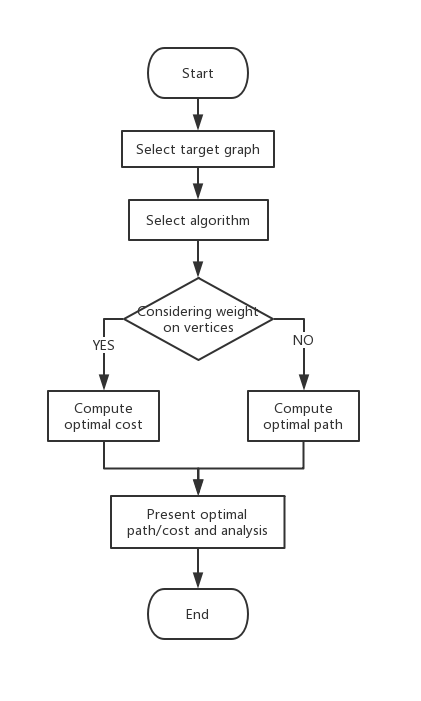
\includegraphics[width=\linewidth]{Systemflowchart.png}
\caption{System Flow Diagram}
\label{fig1}
\end{figure}
\begin{figure}[h]
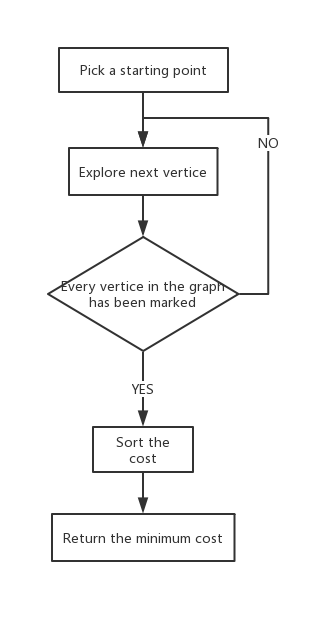
\includegraphics[width=\linewidth]{Method1.jpg}
\caption{Algorithm 1: Exhaustion}
\label{fig2}
\end{figure}
\begin{figure}[h]
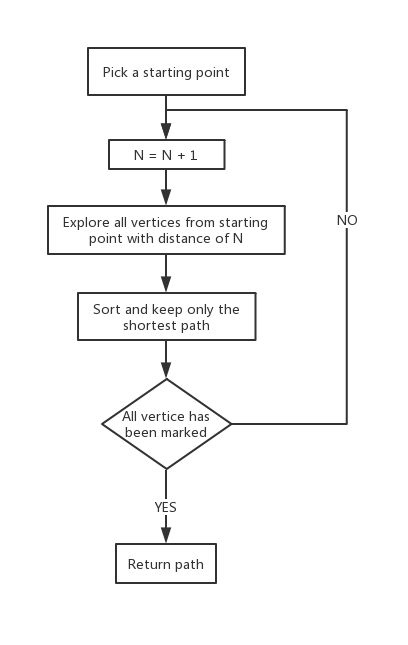
\includegraphics[width=\linewidth]{Method2.png}
\caption{Algorithm 2: Dynamic Programming}
\label{fig3}
\end{figure}
\begin{figure}[h]
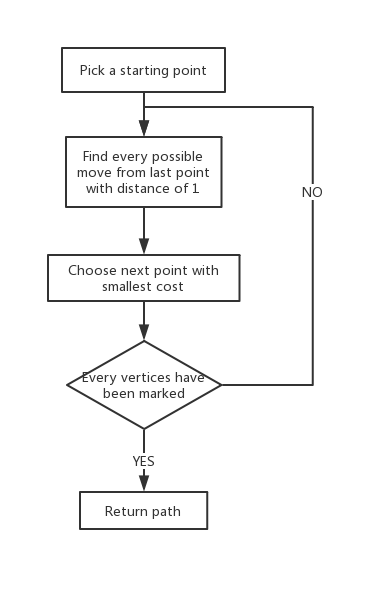
\includegraphics[width=\linewidth]{Method3.png}
\caption{Algorithm 3: Greedy Algorithm}
\label{fig4}
\end{figure}
Please insert your system Flow Diagram here.
\item{ High Level Pseudo Code System Description. }
\\
Initially, a complete directed graph is given. It has weight on edges and vertices.(distance cost and mass cost)
\\
\par
\setlength{\parskip}{0.5\baselineskip}
1. For small n, we can use the easiest method which is exhaustion:
\begin{quote}
\#Set the starting point
\\
\#Generate all permutations of visiting n vertices
\\
\#Keep track of the minimum cost considering weight of both edges and vertices
\\
\#Return the minimum cost and its path
\end{quote}
This method has time and space complexity of O(n!) since there are n! permutations in total(That's why it only works for small n). This method will be used to verify our result using the other two methods.
\par
2. A more realistic and effective way is dynamic programming:
\begin{quote}
\#Set the starting point
\\
\#Start with visiting v=2 vertices in total.(1 starting point and 1 other point)
\\
\#Calculate the cost of each path and store the result.(All vertices visited already, the last vertex visited, total distance cost, total mass cost, mass carried)
\\
\#If more than one path share the same visited vertices and last vertex, only keep the one with minimum cost
\\
\#Continue with v=3 using the result of v=2
\\
\#Repeat the previous steps for v=4, 5, 6... until v=n
\\
\#The last step is adding the edge from the end point back to the starting point and find the minimum cost
\\
\#Return the minimum cost and its path
\end{quote}
This method is much faster than the first one and it should give the correct final answer. But still it is not suitable for n that is too large.
\par
3. An even faster method is greedy algorithm:
\begin{quote}
\#Set the starting point and let end point to be the same point
\\
\#Among all the edges coming out of the end point, find the one with minimum total cost. Include that edge into the path and set the other node of the edge to be new end point
\\
\#Repeat the last step with the new end point until all vertices are visited
\\
\#Return the cost and the path
\end{quote}
This method does not necessarily return the global minimum cost. But with some assumptions, it is still a good approximation and it is really fast!

\item{Algorithms and  Data Structures. }
\\
1. Brute-force approach: explore every possible permutation to find the best solution. Easy but time-consuming.
\\
Data Structures: Graph(Adjacency Matrix), Tree, Array
\par
2. Dynamic programming: Divide the problem into sub-problems. Start with 1 point in the path and continue adding more points until all vertices are visited. Exponential time complexity.
\\
Data Structures: Graph(Adjacency Matrix), Cost Matrix, Binary integer, Array
\par
3. Approximate algorithm: Greedy algorithm always find local minimum cost. It might not give global best solution. But it is fast.
\\
Data Structures: Graph(Adjacency Matrix), Tree, Array
\end{itemize}

\begin{itemize} 
\item{  Flow Diagram Major Constraints.}
Please insert here the integrity constraints:
\begin{itemize} 
\item{ Input Constraint. }
Input graph must be fully connected directed graph.
\end{itemize}
\begin{itemize} 
\item{ Distance Constraint. }
Distance must be positive integer.
\end{itemize}
\begin{itemize} 
\item{ Weight Constraint. }
Weight must be positive integer.
\end{itemize}
\begin{itemize} 
\item{ Output Constraint. }
Output must be an array of path.
\end{itemize}
\end{itemize}

\subsection{Stage3 - The Implementation Stage. }\label{sec: 3 The Implementation Stage.}
%%%%%%%%%%%%%%%%%%%%%%%%%%%%%%%%%%%%%%%%%%%%%%%%%%%%%%%%%%%%%%%%%%%%%%%%%%%%%%%%%%%%%%%%%
\textnormal{
Specify the language and programming environemnt you used for your implementation.
%Building the corresponding relational tables, according to the proposed ER model described in the previous phase %enforcing the different integrity constraints.  
The deliverables for this stage include the following items:
\begin{itemize} 
\item{}
Sample small data snippet. 
%The SQL tables that represent the ER project model, along with at least 3-5 rows of concrete data per table.
\item{}
Sample small output
%The normalization steps for each table, along with explanations/justifications of each normalization step.
\item{}
Working code
%The SQL table after the normalization steps (showing all table attributes).
\item{}
Demo and sample findings
%The SQL statements used to create the SQL tables, including the required triggers as well as the integrity constraints. At %least 2 triggers and 2 of each of the following constraint types have to exist in the project tables overall: 
\begin{itemize} 
\item{}
	Data size: In terms of  RAM size;  Disk Resident?; Streaming ?;  
\item{}
	List the most interestng findings in the data if it is a Data Exploration Project. For other project types consult with your project supervisor what the corresponding outcomes shall be. Concentrate on demonstrating the Usefuness and Novelty of your application.
%Whether some users will be denied access and/or updates to some data according to their roles (for example: student1 %can not access other students' ' grades, so a violation error pops up upon that action. Another example: a sales person %can see an item price, but can not change it, since only a manger can, also a violation error pops up upon that update %attempt).
\end{itemize}
\end{itemize}
}


\subsection{Stage4 -	User Interface. }\label{sec: 4. User Interface.}
%%%%%%%%%%%%%%%%%%%%%%%%%%%%%%%%%%%%%%%%%%%%%%%%%%%%%%%%%%%%%%%%%%%%%%%%%%%%%%%%%%%%%%%%%%%%%%%%%%%%%%%%%%
\textnormal{
Describe a User Interface (UI) to your application along with the related information that will be shown on each interface view (How users will query or navigate the data and view the query or navigation results). The emphasis should be placed on the process a user needs to follow in order to meet a particular information need in a user-friendly manner.
The deliverables for this stage include the following items :
}
\begin{itemize} 
\item{The modes of user interaction with the data (text queries, mouse hovering, and/or mouse clicks ?).} 
\item{The error messages that will pop-up when users access and/or updates are denied   }
\item{The information messages or results that wil pop-up in response to user interface events. }
	
\item{ The error messages in response to data range constraints violations.}
	
\item{ The interface mechanisms that activate different views in order to facilitate data accesses, according to users'  needs. }
	
\item{Each view created must be justified. Any triggers built upon those views should be explained and justified as well. At least one project view should be created with a justification for its use. }	
\end{itemize}

Please insert your deliverables for Stage4 as follows:
\begin{itemize} 
\item{The initial statement to activate your application with the corresponding initial UI screenshot}
	
\item{Two different  sample navigation user paths through the data exemplifying the different modes of interaction and the corresponding screenshots. }

\item{}
	The error messages popping-up when users access and/or updates are denied (along with explanations and examples):
	\begin{itemize} 
	\item{The error message: }
	\item{The error message explanation (upon which violation it takes place): }
	Please insert the error message explanation in here.
	\item{The error message example according to user(s) scenario(s): }
	Please insert the error message example in here.
	 \end{itemize}
\item{}
	The information messages or results that pop-up in response to user interface events.
	\begin{itemize} 
	\item{The information message: }
	Please insert the error message in here.
	\item{The information message explanation and the corresponding event trigger }
	\item{The error message example in response to data range constraints and the coresponding user's scenario }
	Please insert the error message example in here.
	 \end{itemize}
\item{}
	The  interface mechanisms that activate different views.
	\begin{itemize} 
	\item{The interface mechanism: }
	Please insert the interface mechanism here.
	 \end{itemize}
\end{itemize}

\section{Project Highlights.}\label{sec:7. Project Highlights.}
%%%%%%%%%%%%%%%%%%%%%%%%%%%%%%%%%%%%%%%%%%%%%%%%%%%%%%%%%%%%%%%%%%%%%%%%%%%%%%%%%%%%%%%%%%%%%%%%%%%%%%%%%%
\textnormal{
\begin{itemize} 
\item{}
Only working applications will be acceptable at project completion. A running demo shoul be presented to your project advisor at a date to be specified after the second midterm. A version of your application shall be installed in a machine to be specifed later during the semester. Your final submissiom package will also include a final LaTeX report modeled after this document, as well as a Power Point Presentation.
\item{}
The presentation (7 to 8 minutes) should include at least the following items (The order of the slides is important):
\begin{enumerate}
\item{}
Title: Project Names (authors and affiliations)
\item{}
Project Goal
\item{}
Outline of the presentation
\item{}
Description
\item{}
Pictures are essential. Please include Interface snapshots exemplyfing tthe different modes of users's interaction.
\item{}
Project Stumbling Blocks
\item{}
Data collection, Flow Diagram, Integrity Constraints
\item{}
Sample Findings
\item{}
Future Extensions
\item{}
Acknowledgements
\item{}
References and Resources used(libraries, languages, web resources)
\item{}
Demo(3 minutes)
\end{enumerate}
Please follow the sample presentation mock up that is posted on Sakai.
\item{}
By Dec 1 your group should have completed the final submission. This includes a presentation (7 to 8 minutes) to your project advisor as well as a convincing  demo of your project functionalities (3 minutes): every group member should attend the demo (and presentation) indicating clearly  and specifically his/her contribution to the project.  This wil allow us to evaluate all students in a consistent and fair manner.
\item{}
Thank you, and best of luck!
\end{itemize}
}


\bibliographystyle{IEEEtran}
%\bibliography{IEEEabrv,bib_queyroi_abello2013}
%\bibliography{bib_queyroi_abello2013}

\end{document}


